\documentclass[a4paper, 12pt]{extarticle}
\usepackage{geometry}
\usepackage{float}
\usepackage{graphicx}
\usepackage[utf8]{inputenc}
\usepackage{setspace}
\usepackage{lmodern}
\usepackage[hidelinks]{hyperref}
\usepackage{chngcntr}
\usepackage{enumitem,amssymb}
\usepackage{multicol}
\usepackage{float}
\usepackage{tabularx}
%\usepackage{titlesec}
\newcounter{magicrownumbers}
\newcommand\rownumber{\stepcounter{magicrownumbers}\arabic{magicrownumbers}}
%\newcommand \tab[1][1cm]{\hspace*{#1}}
\newlist{todolist}{itemize}{2}
\setlist[todolist]{label=$\square$}
\counterwithin{figure}{section}
\counterwithin{table}{section}
\linespread{1.5}
\newcommand\tab[1][1cm]{\hspace*{#1}}
\geometry{left=20mm,right=20mm,top=20mm,bottom=20mm}
\begin{document}
{
\pagenumbering{roman}
\fontfamily{ptm}\selectfont
\begin{center}	
\textbf{\fontsize{18}{2} \selectfont POST MERGER ANALYSIS OF CUSTOMER SATISFACTION AND LOYALTY - A STUDY ON RECENT MERGER OF ASSOCIATE BANKS OF SBI WITH ITSELF}\\
\tab \\
\textbf{\fontsize{14}{2} \selectfont A PROJECT REPORT}\\
\tab \\
\textbf{\fontsize{14}{2} \selectfont \emph{Submitted by}}\\
\tab \\
\tab \\
{\fontsize{16}{2} \selectfont
\textbf{ADHITHYAN V}}\\
{\fontsize{16}{2} \selectfont \textbf{(2016201002)}}\\
\tab \\
\textbf{\emph{\fontsize{14}{2} \selectfont in partial fulfillment for the award of the degree\\ of}}\\
\tab \\
\textbf{\fontsize{16}{2} \selectfont MASTER OF BUSINESS ADMINISTRATION}\\
\begin{figure}[H]
\centering

\includegraphics[scale=0.5]{anna_univ_logo.jpg}
\end{figure}
\textbf{\fontsize{14}{2} \selectfont DEPARTMENT OF MANAGEMENT STUDIES, \\COLLEGE OF ENGINEERING, GUINDY}\\
\tab \\
\textbf{\fontsize{16}{2} \selectfont ANNA UNIVERSITY : CHENNAI 600 025}\\
{\fontsize{14}{2} \selectfont MAY 2018}\\
\end{center}
	
% bonafide certificate
\newpage
\begin{center}
\textbf{\fontsize{18}{2} \selectfont ANNA UNIVERSITY : CHENNAI 600 025}\\
\tab \\
\textbf{\fontsize{16}{2} \selectfont BONAFIDE CERTIFICATE}\\
\end{center}
Certified that this project report \textbf{"POST MERGER ANALYSIS OF CUSTOMER SATISFACTION AND LOYALTY - A STUDY ON RECENT MERGER OF ASSOCIATE BANKS OF SBI WITH ITSELF"} is the bonafide work of \textbf{"ADHITHYAN V (2016201002)"} who carried out the project work under my supervision. Certified further, that to the best of my knowledge the work reported herein does not form part of any other project work or dissertation on the basis of which a degree or award was conferred on an earlier occasion on this or any other candidate.
\tab \\
\tab \\
\tab \\

\noindent \textbf{SIGNATURE OF HEAD OF THE DEPARTMENT} \hfill \hfill \textbf{SIGNATURE OF GUIDE}\\
\noindent Dr. L. Suganthi B.Tech., MBA., Ph.D., \hfill \hfill Dr.A.Thiruchelvi,\\
\noindent Professor \& Head, \hfill \hfill Asst.Professor,\\
\noindent Department of Management Studies, \hfill \hfill Department of Management Studies,\\
\noindent Anna University, \hfill \hfill Anna University,\\
\noindent Chennnai - 25. \hfill \hfill Chennai - 25.

%acknowledgement
\newpage
\begin{center}
\textbf{\fontsize{16}{2} \selectfont ACKNOWLEDGEMENT}\\
\end{center}
\par I would like to express my sincere gratitude to \textbf{Dr. L. Suganthi}, Head of the Department, and all beloved staffs of Department of Management Studies for instilling confidence in me to carry out this study and extending valuable guidance and encouragement from time to time, without which it would not have been possible to undertake and complete this project.  

\par I wish to thank my project guide \textbf{Dr. A. Thiruchelvi}, Assistant Professor, who has given her support, advice and guidance in completing the project successfully.

%abstract
\newpage
\begin{center}
\textbf{\fontsize{14}{2} \selectfont ABSTRACT}\\
\end{center}
\par Mergers typically involve two relatively equal companies making the mutually beneficial decision to become a single legal entity. They are different from acquisitions, which usually involve a larger company absorbing a smaller company, sometimes against the will of the smaller company's management. Mergers are undertaken to improve long-term shareholder value and overall company performance. They are often done to reduce operating costs, improve market pentration and diversification.
\par A satisfied customer remains loyal and spreads positive word of mouth. Mergers and acquisitions often focus on financial aspects but rarely consider the customer facet of mergers. Studies show that 2/3 rd of mergers fail due to dissatisfied customers.A dissatisfied customer also switches the brand.Merger process are often done without considering the customers. Studies have found that more than half of all mergers fail to deliver the intended improvement in stakeholder value and that customer defections contribute to that high failure rate. Thus, a harmonious integration of the beliefs and values of a merging firm and the ability to integrate organisational cultures is more important to success than the financial or strategic factors. Customer switching also increases post merger. This study aims to find out loyalty and customer satisfaction post merger considering various factors such as demographics, brand image, psychological breach of contract etc taking the recent merger of associate banks of SBI with itself as a case study.

\newpage

\tableofcontents
\listoffigures
\listoftables

\newpage
\pagenumbering{arabic}
%introduction
\section{Introduction}
\par Public Sector Banks (PSBs) are banks where a majority stake (i.e. more than 50 \%) is held by a government. The shares of these banks are listed on stock exchanges. There are a total of 21 PSBs in India.

%\subsection{LIST OF PUBLIC SECTOR BANKS IN INDIA}
%\begin{enumerate}
%\item Allahabad Bank
%\item Andhra Bank
%\item Bank of India
%\item Bank of Baroda
%\item Bank of Maharastra
%\item Canara Bank
%\item Central Bank of India
%\item Corporation Bank
%\item Dena Bank
%\item Indian Bank
%\item Indian Overseas Bank
%\item Oriental Bank of Commerce
%\item Punjab and Sindh Bank
%\item Punjab National Bank
%\item Syndicate Bank
%\item UCO Bank
%\item Union Bank of India
%\item United Bank of India
%\item Vijaya Bank
%\end{enumerate}
%\par SBI and IDBI often mentioned in this list are regarded as PSUs and not as nationalised banks themselves.

\subsection{SBI}
\par The roots of the State Bank of India lie in the first decade of the 19th century, when the Bank of Calcutta later renamed the Bank of Bengal, was established on 2 June 1806. The Bank of Bengal was one of three Presidency banks, the other two being the Bank of Bombay (incorporated on 15 April 1840) and the Bank of Madras (incorporated on 1 July 1843). All three Presidency banks were incorporated as joint stock companies and were the result of royal charters. These three banks received the exclusive right to issue paper currency till 1861 when, with the Paper Currency Act, the right was taken over by the Government of India. The Presidency banks amalgamated on 27 January 1921, and the re-organised banking entity took as its name Imperial Bank of India. The Imperial Bank of India remained a joint stock company but without Government participation.

\par Pursuant to the provisions of the State Bank of India Act of 1955, the Reserve Bank of India, which is India's central bank, acquired a controlling interest in the Imperial Bank of India. On 1 July 1955, the imperial Bank of India became the State Bank of India. In 2008, the Government of India acquired the Reserve Bank of India's stake in SBI so as to remove any conflict of interest because the RBI is the country's banking regulatory authority.

\subsubsection{FORMATION OF SBI AND ASSOCIATE BANKS}
\par The Central Government entered the banking business with the nationalization of the Imperial Bank of India in 1955. This made SBI subsidiaries of eight that had belonged to princely states prior to their nationalization and operational takeover between September 1959 and October 1960, which made eight state banks associates of SBI. This with the first Five Year Plan, which prioritised the development of rural India. The government integrated these banks into the State Bank of India system to expand its rural outreach. In 1963 SBI merged State Bank of Hyderabad (est. 1943) and State Bank of Bikaner (est.1944).A 60\% stake was taken by the Reserve Bank of India and the new bank was named as the State Bank of India. The seven other state banks became the subsidiaries of the new bank in 1959 when the State Bank of India (Subsidiary Banks) Act, 1959 was passed under the Nehru government.

The seven associate banks of SBI are
\begin{enumerate}
\item State Bank of Bikaner and Hyderabad (SBBJ)
\item State Bank of Patiala (SBBJ)
\item State Bank of Mysore (SBM
\item State Bank of Travancore (SBT)
\item State Bank of Hyderabad (SBH)
\item State Bank of Indore (SBI)
\item State Bank of Saurashtra (SBS)
\end{enumerate}

\subsubsection{SHARE HOLDING PATTERN OF SBI}
\begin{table}[H]
\centering
\begin{tabular}{|c|c|}
\hline
Shareholders & Percentage of shares \\
\hline
Promoters (Govt of India) & 61.23 \\
\hline
FIIs GDRs OCBs NRIs & 11.17 \\
\hline
Banks Insurance companies & 10\\
\hline
Mutual funds and UTI & 8.29\\
\hline
Others & 9.31 \\
\hline
\end{tabular}
\caption{SBI - SHAREHOLDING PATTERN}
\end{table}

\subsubsection{MERGERS AND ACQUISTIONS IN BANKING SECTOR}
The banking industry is an important area in which mergers and acquisitions do make enormous financial gains. As a result of changes in the expectation of the corporate customer, banks are now constrained to rethink their business and devise new strategies. The Indian banking sector is going through a process of restricting, mainly driven by pervasive trends such as deregulation, disintermediation, technological progress, innovation and severe competition.To gain competitive cost advantage, consolidation of operation in the form of M\&A is one of the effective strategies widely adopted by the bankers. Mergers in banks are considered for the purpose of:
\begin{enumerate}
\item Expansion/diversification
\item Upgradation of technology
\item Loss making bank merged with another healthy bank for revival
\item Healthy bank merged with another healthy bank to become financially
stronger, to meet competitive pressures
\item Growth in profits
\item Increase market share, etc.
\end{enumerate}
Banks allocate resources and control internal processes by effectively
managing their employees, facilities, expenses, and sources and uses of funds while working to maximize earning assets and total income. M\&A are not new to the Indian banking sector. Between 1961- 2004, 71 mergers took place among various banks in India.
\subsubsection {SBI AND IT'S ASSOCIATES MERGER}
\par According to a gazette notification dated 22 February 2017 , the government said that all shares of these associate banks would cease to exist as individual entities and would merger with SBI. On April 1, 2017 SBT, SBM, SBH, SBBJ and SBP was merged with SBI. This merger has catapulted SBI to top 50 banks in world. It will join the league of top 50 banks in the workd in terms of assets. The total customer base of the bank will reach 37 crores with a branch network of around 24,000 and nearly 59,000 ATMs across the country. The merged entity will have a deposit base of more than Rs 26 lakh crore and advances level of INR 18.50 lakh crore.
\par Post merger, the bank will rationalise its branch network by relocating some of the branches to maximise reach. This will help the bank optimise its operations and improve profitability. As per the bank the merger will enhance productivity, mitigate geographical risks, increase operational efficiency and driver synergies across multiple dimensions while ensuring increased levels of customer delight.

\subsubsection {REASON FOR SBI AND IT'S ASSOCIATES MERGER}
\par \textbf{Govt. Aid to 1 Merged SBI Group :} Firstly the SBI and associates are one of the largest Govt. undertaking of the Central Govt. whom annual allocation of subsidy and contribution towards Bad Debt Recovery and Share Capital has to be made by the Indian Govt. There is practically no sense of giving aid to so many banks separately when it can be given to a single entity. Govt. Aid is for sure to be given to these banks and not just SBI and group but all the banks. So Govt. Aid to a single SBI merged bank will be much easier in terms of accountability.
\par \textbf{Bad loans and inability to recover :} SBI and group is the one of the largest banking sector entities who have crores and crores of Bad Loans which are not recoverable. Some entities Gross NPA has reached up to 20\%. Due to huge bad loans an internal corporate restructuring is required for all the associate group entities, otherwise in upcoming few years, few of them may even not survive in the market.
\par \textbf{Corporate restructuring :} Merger of the group entities of SBI is a way to restructure the Balance Sheet of the entities. Restructuring is required when the entities are facing financial crises or there is a possibility of the entity to not be able to meet out its existing liabilities. In corporate restructuring some liabilities are set off with realisation of assets. In this case, some entities liabilities will be sett off against the higher revalued assets of the other entities in order to make a good and attractive Balance Sheet Size of the merged entity.
\par \textbf{Bigger Bank :}By merging all the associate entities, SBI will become a much bigger and better bank as it will be catering to al large segment of customers as from its current position. It will be able to make many services convenient to the customers through a single bank rather than approaching other associated banks. It will have larger customer base, hence chances of earning good profitability over its deposits. It will have the advantage of Synergy with the associated banks. No high integration cost will be paid since the set-up is almost similar. It will have good asset portfolio. Allover, good report will be created amongst its customers.
\par \textbf{Better management :} Since it will become one big merged Bank, it will have only a management system rather than having different management set-up over the associate banks. Because of single management, efficiency and effectiveness of the business processes will be increased. Single circular will be issued for all the merged Banks for operational and management supervision. Better internal control and system processes will be carries on with all the merged banks
\par \textbf{Better increased recognition :} Those areas where SBi is not having branches but its associate banks are having, upon the merger being effected, the customer confidence and good report will be created because SBI is having a good report for all its customers but the other associate banks are not that good as the SBI. Also, they do not enjoy all those benefits as the SBI. Some sort of change in name from SBI associates to SBI will have a good market impression and will generate goodwill.

\subsubsection{ADVANTAGES OF MERGER}
\begin{itemize}
\item The most common reason for firms to enter into merger and acquisition is to merge their power and control over the markets.
\item Another advantage is Synergy that is the magic power that allow for increased value efficiencies of the new entity and it takes the shape of returns enrichment and cost savings.
\item Economies of scale is formed by sharing the resources and services. Union of 2 firm's leads in overall cost reduction giving a competitive advantage, that is feasible as a result of raised buying power and longer production runs.
\item Decrease of risk using innovative techniques of managing financial risk.
\item To become competitive, firms have to be compelled to be peak of technological developments and their dealing applications. By M\&A of a small business with unique technologies, a large company will retain or grow a competitive edge.
\item The biggest advantage is tax benefits. Financial advantages might instigate mergers and corporations will fully build use of tax- shields, increase monetary leverage and utilize alternative tax benefits 
\end{itemize}

\subsubsection{DISADVANTAGES OF MERGER}
\begin{itemize}
\item Loss of experienced workers aside from workers in leadership positions. This kind of loss inevitably involves loss of business understand and on the other hand that will be worrying to exchange or will exclusively get replaced at nice value.
\item As a result of M\&A, employees of the small merging firm may require exhaustive re-skilling.
\item Company will face major difficulties thanks to frictions and internal competition that may occur among the staff of the united companies. There is conjointly risk of getting surplus employees in some departments.
\item Merging two firms that are doing similar activities may mean duplication and over capability within the company that may need retrenchments.
\item Increase in costs might result if the right management of modification and also the implementation of the merger and acquisition dealing are delayed.
\item The uncertainty with respect to the approval of the merger by proper assurances.
\item In many events, the return of the share of the company that caused buyouts of other company was less than the return of the sector as a whole.
\end{itemize}

\subsection{PROBLEM STATEMENT}
\par A satisfied customer remains loyal and spreads positive word of mouth. Mergers and acquisitions often focus on financial aspects but rarely consider the customer facet of mergers. Studies show that 2/3 rd of mergers fail due to dissatisfied customers.A dissatisfied customer also switches the brand.Merger process are often done without considering the customers. Studies have found that more than half of all mergers fail to deliver the intended improvement in stakeholder value and that customer defections contribute to that high failure rate. Thus, a harmonious integration of the beliefs and values of a merging firm and the ability to integrate organisational cultures is more important to success than the financial or strategic factors. Customer switching also increases post merger. This study aims to find out loyalty and customer satisfaction post merger considering various factors such as demographics, brand image, psychological breach of contract etc taking the recent merger of associate banks of SBI with itself as a case study.

\subsection{NEED FOR THE STUDY}
\par Most of the merger effectiveness are assessed based on financial performance, synergy. Rarely the studies assess the effectiveness of merger from customer perspective.The success of merger depends not only on financial aspects but also creating value for its stakeholders. There has been lot of failed mergers because most of the mergers didn't consider human aspects of merger. This study is important to find out level of service changes in banks post merger and their impact on customer satisfaction and loyalty due to service changes and psychological breach of contract. A psychological contract breach refers to subjective perception that other party has failed to adequately fulfill promised obligations. This study will also be useful to assess the effectiveness of merger from customer point of view.

\subsection{SCOPE OF THE STUDY}
The associate banks of State Bank of India (SBI) that merged with it recently are State Bank of Bikaner and Hyderabad (SBBJ), State Bank of Mysore (SBM), State Bank of Travancore (SBT), State Bank of Hyderabad (SBH), State Bank of Patiala (SBP). This study is applicable to most of the major cities like Chennai, Bangalore, Hyderabad and Pollachi.

\subsection{OBJECTIVES}
\subsubsection{PRIMARY OBJECTIVE}
\begin{itemize}
\item To find out customer satisfaction and loyalty post merger in SBI.
\end{itemize}
\subsubsection{SECONDARY OBJECTIVE}
\begin{itemize}
\item To find out benefits of merger from customer perspective.
\item To find out various issues faced by customer post merger.
\end{itemize}

\subsection{HYPOTHESIS}
\begin{itemize}
\item \textbf{H1} - Psychological Contract Violation has negative influence on customer satisfaction.
\item \textbf{H2} - Service performance is a determinant of Overall Service
\item \textbf{H3} - Overall service has a positive impact on customer satisfaction
\item \textbf{H4} - Customer satisfaction has positive influence on customer loyalty.
\end{itemize}

\newpage
\section{LITERATURE REVIEW}
\subsection{MERGERS \& ACQUISITIONS IN BANKS}
\begin{itemize}
\item Trust and satisfaction increases customers intention to reuse the product. Psychological contract violation affects customer satisfaction and their intention to use the product. \emph{(Psychological contract violation and customer intention to reuse online retailers - Neeru Malhotra a, Sunil Sahadev b, Keyoor Purani ., 2017)}
\item Customer often compare the pre and post merger service changes. Nostalgia plays an important role in this. \emph{(Effect of nostalgia on customer loyalty to Brand Post-merger / acquistions – Ana Carolina Toledo, Evandro Luiz Lopes., 2016)}
\item Various factors like satisfaction, trustworthiness, image and relationship affect customer loyalty and firms should maintain them at any cost – \emph{( Affecting customer loyalty: Do different factors have various influences in different loyalty levels – Andres kussik  - 2007)}
\item Sangita,M (2015) opines that the large banks are not in a position to takeover small banks as they face the same problems of their potential targets and he also said the merger of any bank with SBI can only be done if the performance of the particular bank matches with the standards of SBI. 
\item Tiwari.,D. (2014). said that the decision of mergers of bank would be based on political conditions rather than on economic conditions and it would also create overlapping among various state owned banks in terms of branches and clients.
\item Tripathy., D \& Chatterjee S.(2014) The author explains that the consolidation of banks should support an expected recovery in Asia's third largest economy by creating strong lenders which help to control the growth of bad loans and would make the credit availability easier. 
\end{itemize}
\subsection{PSYCHOLOGICAL CONTRACT VIOLATION}
\par A psychological contract can be defined as perceived mutual obligations between two parties that are to be fulfilled by one party or other (Rousseau \& Tijoriwala, 1998). Psychological contracts are based on perceived promises and arise when one party is obligated to perform certain behaviour (Rousseau, 1995). From a customer's perspective, psychological contracts comprise the customer's perceptual beliefs about the seller's contractual obligations. So customer's individual perception of psychological contract violation (PCV) may occur if they think they are not getting what has been promised by a contractual agreement (Theotokis, Pramatari, \& Tsiros, 2012). So, PCV damage the bond between customer and seller and has a negative impact on customer satisfaction and loyalty (Malhotra, Sahadev \& Purani, 2017). While PCV has been studied mainly in the context of employee organization relationships, Pavlou and Gefen (2005) examine PCV in customer seller relationships. Every customer-seller interaction can be characterized by the psychological contract that features the customer's perceptual beliefs about the seller's contractual obligations, which may not be included in the formal legal terms of the exchange.

\par According to psychological contract theory, violations are inevitable in contractual relationships. When one party fails to fulfil obligation violation may occur. Thus, in a customer seller scenario, PCV occurs when customer thinks that seller's failure has violated the psychological contract (Robinson \& Morrison, 1997). Customers may perceive PCV even when the actual contract rules may have not been violated. PCV can also be caused by misunderstandings regarding the contractual obligations. PCV is rooted in two contributing factors: reneging and incongruence. Reneging is intentional failure to meet obligations. It can be readily observable.  When a seller wilfully defaults a obligation such shipping a defective product, misrepresenting advertisements. This can be done by the seller for the purpose of cutting costs and reaping profits (Robinson \& Morrison, 2000).
Incongruence refers to perceived violation of psychological contract. According to Morrison and Robinson (1997), three factors contribute to incongruence: ambiguity in terms of relationship, prior experiences, and lack of communication between customer and seller.
\subsection{CUSTOMER SATISFACTION}
\par Customer satisfaction has been defined in various ways, but the conceptualization, which appears to have achieved the widest acceptance, is that satisfaction is a post-choice evaluative judgment of a specific transaction (Bastos and Gallego, 2008). Customer satisfaction is the result of a customer's perception of the value received in a transaction or relationship where value equals perceived service quality relative to price and customer acquisition costs (Hallowell, 1996; Heskett et al., 1990; Blanchard and Galloway, 1994). While the literature contains significant differences in the definition of satisfaction, all the definitions share some common elements (Giese and Cote, 2002). When examined as a whole, three general components can be identified:
\begin{enumerate}
\item Consumer satisfaction is a response (emotional or cognitive);
\item The response pertains to a particular focus (expectations, product, consumption experience, etc.);
\item The response occurs at a particular time (after consumption, after choice, based on accumulated
\end{enumerate}
experience, etc).
\subsection{LOYALTY}
\par Emotional loyalty is much stronger and longer lasting than beha- vioral loyalty. It's an enduring desire to maintain a valued relation- ship. The relationship is so important for the customer that he or she makes maximum efforts to maintain it. (Morgan et al. 1995: 24; Reichheld 2003: 9; Moorman et al. 1992: 316). Highly bonded customers will buy repeatedly from a provider to which they are bonded, recommend that provider to others, and strongly defend these choices to others insisting that they have chosen the best product or service. (Butz et al. 1996: 65). As suggested by several researchers (Kumar and Shah, 2004; Blak and Parks, 2003; Bell et al, 2005 and Dean, 2007) there are two types of loyalty; behavioral and attitudinal loyalty. The behavioral aspects of the customer loyalty were characterized in terms of repurchase intentions, word-of-mouth communication, and recommendations of the organization (Nadiri, et al. 2008; Karatepe and Ekiz, 2004; Yi, 1990; Zeithaml et al., 1996). Liu-Thompkins, et al (2010) defined attitudinal loyalty as a favorable evaluation that is held with sufficient strength and stability to promote a repeatedly favorable response towards a product/brand or a store. According to Kumar and Shah (2004) Consumer loyalty seems to be based on a collection of factors. The first is trust. Consumers must trust the vendor or product they encounter. Second, the transaction or relationship must have a positive perceived value greater than that supplied by competitors. Third, if marketers build on the first two factors, they may be able to create a level of positive customer emotional attachment. That emotional response may be commitment to their brands that is resistant to change (Pitta, et al, 2006). Today, every industry offers a variety of loyalty schemes aiming at differentiating one competitor from another (Butscher, 1999).

\subsection{SENTIMENT ANALYSIS}
Sentiment analysis has limited ability to detect extreme ratings explicitly assigned by reviewers (Lak and Tureken, 2014).



\subsection{RESEARCH GAP}
This study has not been conducted before. This is the first such attempt to assess merger effectiveness from customer point of view. Psychological breach of contract in banking sector from customer perspective have not been studied before. Studies on this topic has been done on e-Commerce.

\subsection{PROPOSED MODEL}
\begin{figure}[H]
\centering
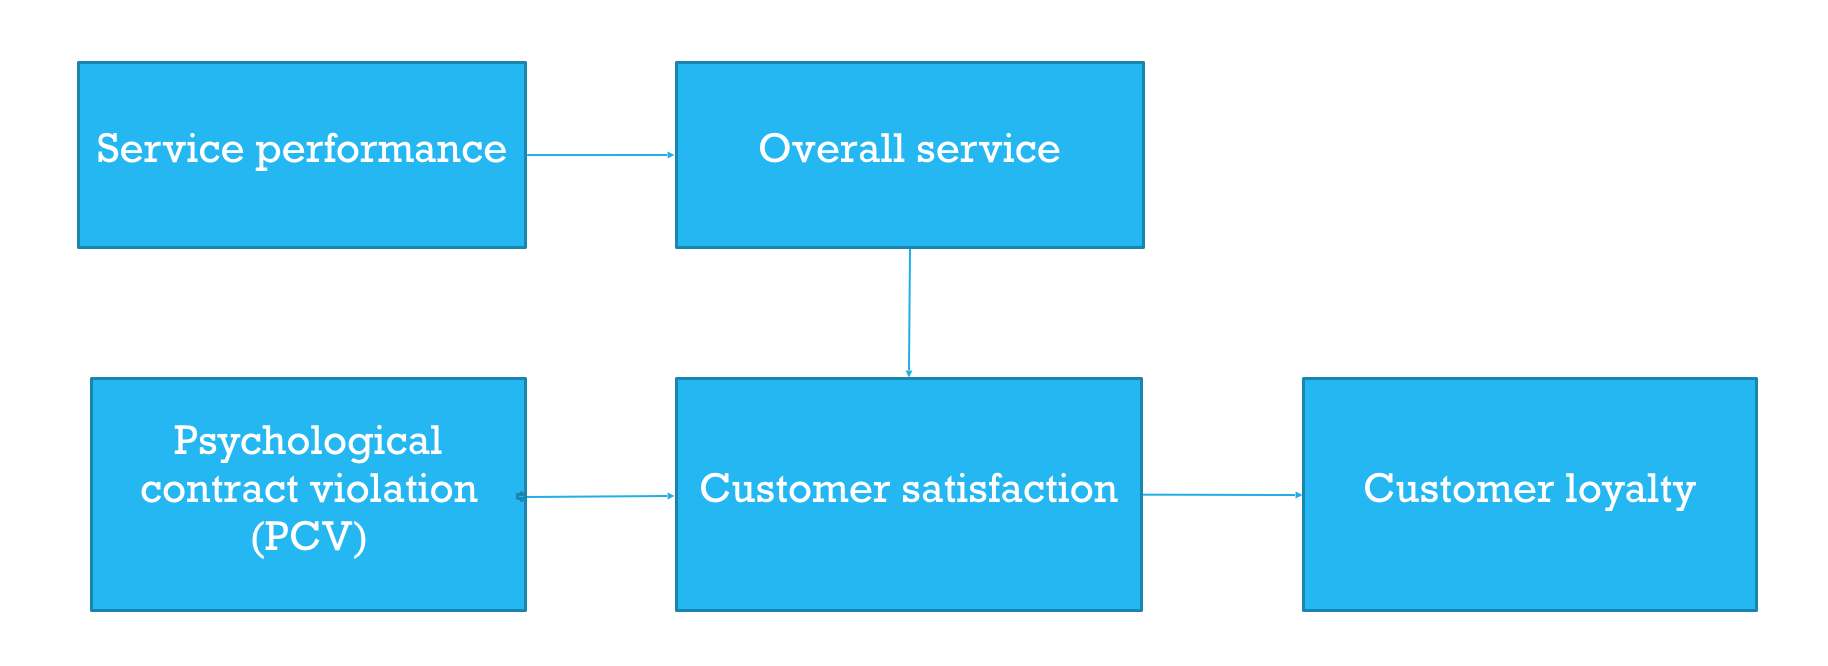
\includegraphics[scale=0.5]{model.png}
\caption {PROPOSED MODEL}
\end{figure}

\newpage

\section{METHODOLOGY}
\subsection{RESEARCH DESIGN}
The research problem has already been identified and described in chapter 1. Based on this, research design and methodology have been defined and data collection has been carried out.

\subsection{DATA COLLECTION}
\par The data is collected using survey method using a questionnaire. Convenience sampling is followed in this study. The research units comprised of customers of State Bank of India (SBI) after merger; that is, previously, they were employees of State Bank of Mysore (SBM), State Bank of Hyderabad (SBH), State Bank of Travancore (SBT). The target population consisted of all customers belonging to the recently- merged SBI.
\subsection{SAMPLING TECHNIQUE}
The sample size is 100. Non-probability sampling was used to obtain data. Particularly convenience sampling was used to collect data.
\subsection{PRIMARY DATA}
\par Around 100 responses were obtained. Data was collected in both online and offline modes. For online mode data collection, twitter was used as a medium to convey about the survey. Tweeters who have mentioned any of the above banks in their tweets were identified based on the tweet content and they were contacted using Twitter mentions to obtain data. Around 25 samples were collected from offline mode. The rest of the data was collected using online mode.
\subsection{SECONDARY DATA}
In addition, we crawled the Mouthshut.com sites to obtain reviews and ratings of SBT, SBBJ, SBM, SBH and SBP customers. Out of the 5 associate banks merged, SBT, SBM and SBBJ were listed in BSE. The historic prices of those stocks along with SBI for the period before and after merger were obtained from BSE site.

\subsection{INSTRUMENT}
The questionnaire consists of 27 questions and 8 standard scales were used.PCV was measured using Psycones (2005)  5 point scale. Service performance was measured using Cronin, Brady, Thomas, Hult (2000)  5 point scale. Customer satisfaction was measured using 
Angelova , Zekiri (2011)  5 point scale and Cronin, Brady, Thomas, Hult (2000)  5 point scale. Customer loyalty was measured using Danaher, Haddrell (1996) 4 point scale and Angelova , Zekiri (2011) 5 point scale. 24 items were transformed into statements rated on a five  point Likert scale from Strongly disagree to Strongly agree and Very Low to Very High etc. 3 items in loyalty were measured using 4 point scale.

\subsection{DATA PREPARATION}
The data collected was checked for missing values and the complete dataset was used for comprehensive analysis.

\subsection{TECHNIQUES USED}
For primary data statistical analyses were made using SPSS. Descriptive statistics, regression analysis were performed. The statistical techniques to be used here also include scale reliability assessment using Cronbach's Alpha (Cronbach, 1951). Each of the hypotheses (H1 to H5) is tested using linear regression analysis. It helps to apprehend how the distinctive value of the dependent variable changes when any one of the independent variables is varied, while the other independent variables are held fixed.

Reviews and ratings from mouthshut.com was obtained using a python script. The obtained data was analysed using R. Sentiment analysis and correlation of ratings vs review content were performed.
 

\subsection{LIMITATIONS}
The survey was carried out in the premises of SBI and SBT (pollachi), SBM and SBH (Coimbatore) SBH, SBH (Thiruvanmiyur). In addition online survey was also conducted and the responses obtained was from places like Chennai, Hyderabad, Trichy and Bangalore. Most of the responses were from male. So this survey has gender bias. In addition online mode responses may not be understood properly by the respondents due to lack of instant communication. 

\subsection{SUMMARY}
The hypotheses are formulated and research design has been explained and data has been collected using survey method with a help of a questionnaire. After screening the data collected to have complete datasets, analysis and interpretation are carried out with the help of SPSS. The data along with the interpretations are discussed in the subsequent chapters.

%data analysis
\newpage
\section{DATA ANALYSIS}
\subsection{INTRODUCTION}
This chapter presents the results of descriptive statistics, tests of reliability, comparison of means, regression. Firstly, it presents the results of preliminary analyses such as reliability of the measures, descriptive statistics, background and demographic differences in the study variables. Finally, it depicts the summary of results.

\subsection{SCALE RELIABLITY}
Reliability testing concerns the extent to which the measuring procedures yield the same results on repeated trials. Reliability analysis of the measures/scales is generally carried out by item-to-total correlation and Cronbach's alpha. In this research, the Cronbach's  alpha was used to test the reliability.
\begin{table}[H]
\centering
\begin{tabular}{|c|c|c|}
\hline
\textbf{Scale name} & \textbf{Cronbach $\alpha$} & \textbf{No of items}\\
\hline
Psychological Contract Violation & \textbf{0.89} & 8\\
\hline
Service Performance & \textbf{0.712} & 10\\
\hline
Customer Satisfaction & \textbf{0.96} & 4\\
\hline
Customer Loyalty & \textbf{0.927} & 5 \\
\hline
\end{tabular}
\caption{Reliablity of the measures}
\end{table}

\par According to Nunally(1978), Cronbach's coefficient alphas above the threshold value of 0.7 is sufficient to prove the reliability of the scales. It is evident from the table that the scales used are internally reliable. From table it is clear that all scales are reliable. Customer satisfaction and customer loyalty scales are highly reliable since their value is greater than 0.9.

\subsection{DEMOGRAPHICS}
Out of 100 responses 84 were male (83.2 \%) and 17(16.8 \%) were female. The age distribution of respondents is shown in figure.
\begin{figure}[H]
\centering
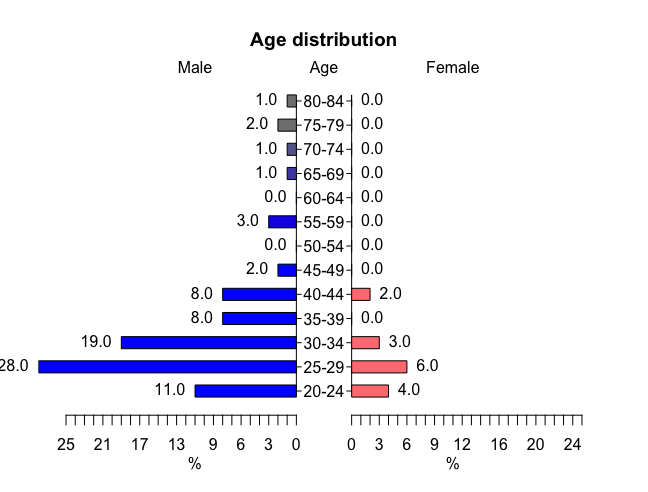
\includegraphics[scale=0.7]{age.png}
\caption{Age distribution of respondents}
\end{figure}
It can be seen that 34 (33.6\%) respondents belong to the age group 25 to 29 while 22 (21.7\%) respondents belong to the age group 30-34. They both form the majority of responses. 15 (14.8 \%) respondents belong to age group 20-24. 8 respondents belong to 35-39 age group. Another 8 respondents belong to age group 40-44.

\subsubsection{ACCOUNT OPENING TIMELINE}
96\% of respondents have opened an account in any of the 5 associate banks before 2017. It indicates that they are associated with bank even before merger. Since our target is to find the post merger customer satisfaction and loyalty, this percentage is very strong to proceed with our analysis.

\subsubsection{LOCATION}
Majority of respondents are from Hyderabad (21\%), followed by Chennai (11\%), Bangalore (10\%) and Pune, Pollachi (8\%). The remaining responses were obtained from places like  Trichy, Mumbai, Pune, Ahmedabad etc.

\subsection{DESCRIPTIVE STATISTICS}
A summary of the descriptive statistics for all study variables is presented in following table. The descriptive statistics presents the mean, the range, minimum and maximum values and standard deviation. The mean age of the respondents (N = 100) was 35.3 years (SD = 12.37). 

\begin{table}[H]
\centering
\begin{tabular}{|c|c|c|c|}
\hline
Item & \textbf{Mean} & \textbf{SD} & N \\
\hline
Customer satisfaction & 2.968 & 1.37 & 100 \\
\hline
PCV & 3.06 & 0.98 & 100 \\
\hline
Overall service & 2.80 & 1.49 & 100 \\
\hline
Service performance & 3.01 & 1.0428 & 100 \\
\hline
Loyalty & 3.07 & .368 & 100 \\
\hline
\end{tabular}
\caption{Descriptive Statistics - Overall}
\end{table} 

\begin{table}[H]
\centering
\begin{tabular}{|c|c|c|}
\hline
Question & Mean & SD \\
\hline
\textbf{ I feel happy about the merger.} & 3.6 & 1.26 \\
\hline
\textbf{ I feel pleased about the merger} & 4.2 & 1.19 \\
\hline
\textbf{ I feel disappointed about the merger } & 2.4 & 1.1 \\
\hline
\textbf{ I feel violated about the merger} & 1.9 & 0.5 \\
\hline
\textbf{ I feel grateful about the merger} & 3.2 & 1.01 \\
\hline
\textbf{ I have difficulty in obtaining information post merger. } & 2.73 & 1.4 \\
\hline
\textbf{ I find difficult to commute.} & 2.3 & 1.47 \\
\hline    
\textbf{ I lost my personal care / identity after merger. } & 4.2 & 1.2 \\
\hline
\textbf{ Time required to avail a service.} & 3.3 & 1.3 \\
\hline
\textbf{ Effort taken to receive a service.}  & 3.5 & 1.42 \\ 
\hline
\textbf{ Employees provide consistent service.}  & 3.15 & 0.6\\  
\hline
\textbf{ Employees are willing and provide service in a timely manner.} & 3.19 & 1.244\\
\hline
\textbf{ Employees are approachable and easy to contact.} & 3.08 & 0.309\\   
\hline
\textbf{ Employees are courteous, polite and respectful.} & 4.03 & 0.8 \\
\hline
\textbf{ Employees listen and speak to me in  a language I understand.} & 2.05 & 0.994 \\
\hline
\textbf{ Employees are trustworthy, honest and believable.} & 3.05 & 0.506 \\
\hline
\textbf{ Employees make effort to understand my needs.} & 2.7 & 1 \\
\hline
\textbf{ Physical facilities and employees are neat and clean.} & 1.5 & 0.876\\
\hline
\textbf{ The overall ability of bank to satisfy my needs and wants is.} & 3.65 & 1.445 \\
\hline
\textbf{ Overall satisfaction level} & 2.85 & 2.3 \\
\hline
\textbf{ To what extent, service has met expectation ?} & 3.75 & 1.4 \\
\hline
\textbf{ Compare the current service with before merger.} & 2.3 & 1.363 \\
\hline
\textbf{ Would you recommend to a friend / relatives?} & 2.2 & 1.19 \\
\hline
\textbf{ Will you avail service continuosly ?} & 2.5 & 1.2 \\
\hline
\textbf{ Will you open account again ?} & 1.14 & 1.18 \\
\hline
\textbf{ I had a problem or negative experience after merger?} & 3.9 & 0.561 \\
\hline
\textbf{ Given an option to switch, I will switch to other banks.} & 4.43 & 1.525 \\
\hline
\end{tabular}
\caption{Descriptive statistics - Individual}
\end{table}

\subsection{INDIVIDUAL INTERPRETATION}
 
\par \textbf{ I feel happy about the merger.} \\
35\% have given 4 and 32\% have given 5. This indicates 67\% of people felt happy about the merger.

\par \textbf{ I feel pleased about the merger} \\
43\% have rated 4 and 24\% have rated 5. This indicates they are all pleased with merger.\\

\par \textbf{ I feel disappointed about the merger } \\
Majority 35\% of respondents have given 1 showing that they are not at all disappointed due to merger.\\

\par \textbf{ I feel violated about the merger} \\
Majority 39\% have rated 1 showing they do not feel violated due to merger.\\

\textbf{ I feel grateful about the merger}  \\
 45\% have rated 3 followed by 27\% rating 4 indicating that they are neutral regarding this.\\

\textbf{ I have difficulty in obtaining information post merger. } \\
25\% and 28\% have rated 1 and 2 respectively showing that they have somewhat difficulty in obtaining information after merger.\\

\par \textbf{ I find difficult to commute.} \\
 Majority 34\% have responded that they do not have any commuting issues.    

\par \textbf{ I lost my personal care / identity after merger. }  \\
\begin{table}[H]
\centering
\begin{tabular}{|c|c|}
\hline
Scale & Response \% \\
\hline
1 - Not at all & 23 \% \\
\hline
2 - Somewhat & 21 \% \\
\hline
3 - Neutral & 21 \% \\
\hline
4 - Some extent & 23 \% \\
\hline
5 - Very great extent & 15 \% \\
\hline
\end{tabular}
\caption{Loss of identity - responses}
\label{table:identity_loss}
\end{table}
As we can see from table ~\ref{table:identity_loss}, people have rated 1 and 4 mostly followed by 2 and 3, indicating that some people have felt identity loss while some people have not felt identity loss. \\
\newpage
\par \textbf{ Time required to avail a service.} \\
27\% felt that time was very high closely followed by 25\% respondents who felt that time was very same.\\

\par \textbf{ Effort taken to receive a service.} \\ 
29\% felt that effort taken to receive a service was very high.\\

\par \textbf{ Employees provide consistent service.} \\  
31\% have rated 2 indicating that employees consistency of providing service is high. \\

\par \textbf{ Employees are willing and provide service in a timely manner.} \\
There was mixed response for this with 23\% of people rating 2 and 3 indicating that employees had high willingness and provided service in a timely manner. \\

\par \textbf{ Employees are approachable and easy to contact.} \\   
Majority 30\% indicated that employees are highly approachable and easy to contact. \\

\par \textbf{ Employees are courteous, polite and respectful.} \\
27\% of rated 3 indicating that employees politenss, courteousness and respectfulness were same. \\

\par \textbf{ Employees listen and speak to me in  a language I understand.} \\
33\% rated 1 and 43\% rated 2 indicting that employees speak in a language that customers understand. \\

\par \textbf{ Employees are trustworthy, honest and believable.}  \\
30\% rated 2 while 25\% rated 3 indicating that above attribute was high - same. \\

\par \textbf{ Employees make effort to understand my needs.} \\
30 of people felt employees put high amount of effort to understand customers needs. \\

\par \textbf{ Physical facilities and employees are neat and clean.}\\
46\% rated 1 and 41\% rated 2 indicating that physical facilities were highly neat and clean. \\

\par \textbf{ The overall ability of bank to satisfy my needs and wants is.} \\
28\% rated 5 indicating that ability of bank to satisfy needs and want is very low.\\

\par \textbf{ Overall satisfaction level}  \\
Majority 30\% of people stated that they were very dissatisfied with the bank. \\

\par \textbf{ To what extent, service has met expectation ?}  \\
31\% indicated that the servie was much worse than expectation. \\

\par \textbf{ Compare the current service with before merger.}  \\
29\% indicated that they cannot differentiate between pre and post merger. \\

\par \textbf{ Would you recommend to a friend / relatives?}  \\
42\% said that they wont recommend to a friend. \\

\par \textbf{ Will you avail service continuosly ?}  \\
32\% said that they will avail service continuosly. \\

\par \textbf{ Will you open account again ?} \\
48\% indicated that they wont open account again in the bank.

\par \textbf{ I had a problem or negative experience after merger?}  \\
31\% of respondents strongly agreed that they had a negative experience at some point with the bank.\\

\par \textbf{ Given an option to switch, I will switch to other banks.} \\
38\% strongly agreed that they will switch to other banks, if an option is provided.



\subsection{REGRESSION ANALYSIS}
All the proposed hypotheses are tested using regression analysis and the results are tabulated and interpreted in this section. A summary of test results are presented in following table.

\begin{table}[H]
\centering
\begin{tabular}{|c|c|c|c|c|c|}
\hline
Hypothesis no & Std coefficient $\beta$  & R squared & Adjusted R square & F & Results \\
\hline
\textbf{H1} & -0.662 & 0.407 & 0.401 & 67.807 & \textbf{Accepted} \\
\hline
\textbf{H2} & -0.830 & 0.744 & 0.554 & 123.009 & \textbf{Rejected} \\
\hline
\textbf{H3} & 0.907 & 0.9 & 0.899 & 893.550 & \textbf{Accepted} \\
\hline
\textbf{H4} & 0.602 & 0.157 & 0.148 & 18.370 & \textbf{Accepted} \\
\hline 
\end{tabular}
\caption{Regression results}
\end{table}
\newpage
\par \textbf{H1 - Psychological contract breach has a negative influence on customer satisfaction}\\
\begin{figure}[H]
\centering
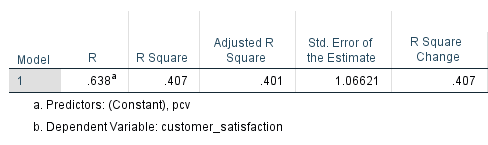
\includegraphics[scale=1]{pcv_vs_customer_satisfaction.png}
\caption{Regression results - H1}
\end{figure}

\begin{figure}[H]
\centering
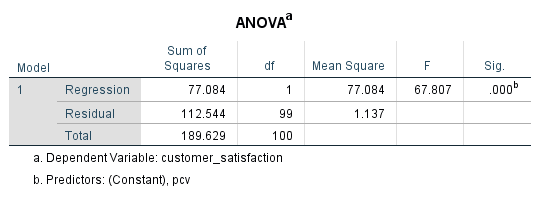
\includegraphics[scale=1]{anova_pcv_cs.png}
\caption{Anova - H1}
\end{figure}

PCV and customer satisfaction are negatively correlated. (-0.662). This indicates as customer perceives more PCV, his satisfaction gets affected. SO H1 is accepted.
PCV influences 41\% of variance in customer satisfaction.\\

\par \textbf{H2 - Service performance is a determinant of overall service.}\\
\begin{figure}[H]
\centering
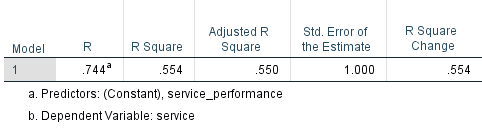
\includegraphics[scale=1]{service_performance_vs_service.png}
\caption{Regression results - H2}
\end{figure}

Service performance explains 55.4\% of variance in overall service.Service performance is negatively correlated with overall service. This indicates overall service doesn't depend on service performance. H2 is rejected.

\begin{figure}[H]
\centering
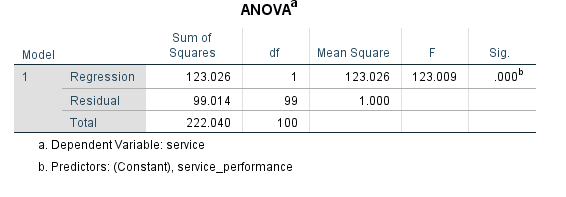
\includegraphics[scale=1]{anova_s_sp.png}
\caption{Anova - H2}
\end{figure}

\par \textbf{H3 - Overall service has a positive impact on customer satisfaction}\\
\begin{figure}[H]
\centering
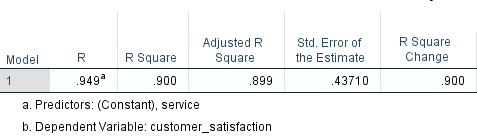
\includegraphics[scale=1]{sp_vs_cs.png}
\caption{Regression results - H3}
\end{figure}

Overall service has a correlation with customer satisfaction. As overall service increases, customer satisfaction tends to increase. H3 is accepted.
Overall service explains 89.9\% variance in customer satisfaction.

\begin{figure}[H]
\centering
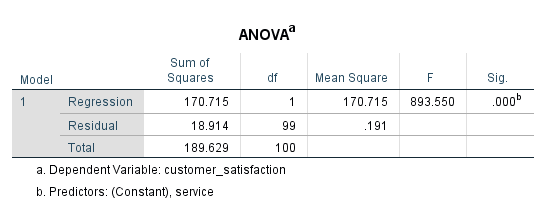
\includegraphics[scale=1]{anova_css.png}
\caption{Anova - H3}
\end{figure}

\newpage
\par \textbf{H4 - Customer satisfaction has a positive influence on customer loyalty.}\\
\begin{figure}[H]
\centering
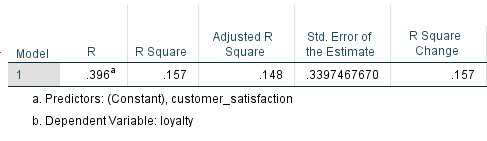
\includegraphics[scale=1]{customer_satisfaction_vs_loyalty.png}
\caption{Regression results - H4}
\end{figure}
\begin{figure}[H]
\centering
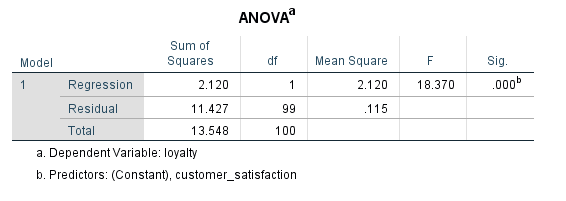
\includegraphics[scale=1]{anova_cs_lo.png}
\caption{Anova - H4}
\end{figure}

Customer satisfaction and loyalty are postively correlated. This indicates a satisfied customer will be more loyal to the bank and spreads word of mouth. H4 is accepted.Customer satisfaction influences 14.8\% of variance in loyalty.

\subsection{CUSTOMER SATISFACTION INDEX}
The American Customer Satisfaction Index (ACSI) is an economic indicator that measures the satisfaction of consumers across the U.S. economy. It is produced by the American Customer Satisfaction Index (ACSI LLC) based in Ann Arbor, Michigan.

\subsection{CUSTOMER SATISFACTION INDEX CALCULATION}
A company's ACSI score is derived from three manifest variables (i.e. survey questions) within the ACSI questionnaire, each rated on a 1-10 scale by the respondents interviewed for that company, government agency, or other organization.

\begin{table}[H]
\centering
\begin{tabular}{|c|c|c|}
\hline
\textbf{Manifest variable} & 1 & 10 \\
\hline
Overall Satisfaction (X1) & Very dissatisfied & Very satisfied \\
\hline
Expectancy disconfirmation (X2) & Falls short of expectation & Exceeds your expectation \\
\hline
Comparison to an ideal (X3) & Not very close to ideal & Very close to the ideal\\
\hline
\end{tabular}
\caption{CUSTOMER SATISFACTION INDEX - CALCULATION}
\end{table}
The 0-100 ACSI score is estimated using the mean for each variable from the n responses for that company (X1, X2, X3), along with the weights for each question as calculated within the ACSI structural equation model (W1, W2, W3):\\ 
\[ (((X1*W1)+(X2*W2)+(X3*W3))-1)/9*100 \]
\par The state of Ohio uses the following weights: \\
\[ ((Satisfaction-1)*.3885 + (Expectancy-1)*.3190 + (Performance-1)*.2925) / 9 * 100 \]
\textbf{\emph{Applying our values, ACSI score was found to be 43.78.}}

\subsection{SECONDARY DATA ANALYSIS - mouthshut.com REVIEWS ANALYSIS}
\subsubsection{RATINGS ANALYSIS}
A total of 199 reviews along with ratings and date of review of SBT, SBM, SBBJ, SBP and SBH were crawled from mouthshut.com.

\begin{table}[H]
\centering
\begin{tabular}{|c|c|}
\hline
Rating & count \\
\hline
1 & 71 \\
\hline
2 & 31 \\
\hline
3 & 23 \\
\hline
4 & 38 \\
\hline
5 & 36 \\
\hline
\end{tabular}
\caption{Ratings distribution}
\end{table}{H}
\begin{figure}[H]
\centering
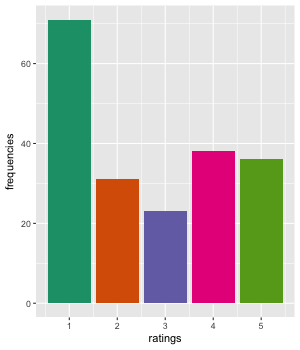
\includegraphics[scale=1]{ratings_distribution.png}
\caption{Ratings distribution}
\end{figure}

The ratings analysis shows that most of the people have given 1 stars (35.6\%), followed by 4 stars (19.1\%) and 5 stars (18.2\%). When 4 and 5 stars are combined we get a percentage of 37.3\% which surpasses the percentage of 1 star ratings. 
\begin{figure}[H]
\centering
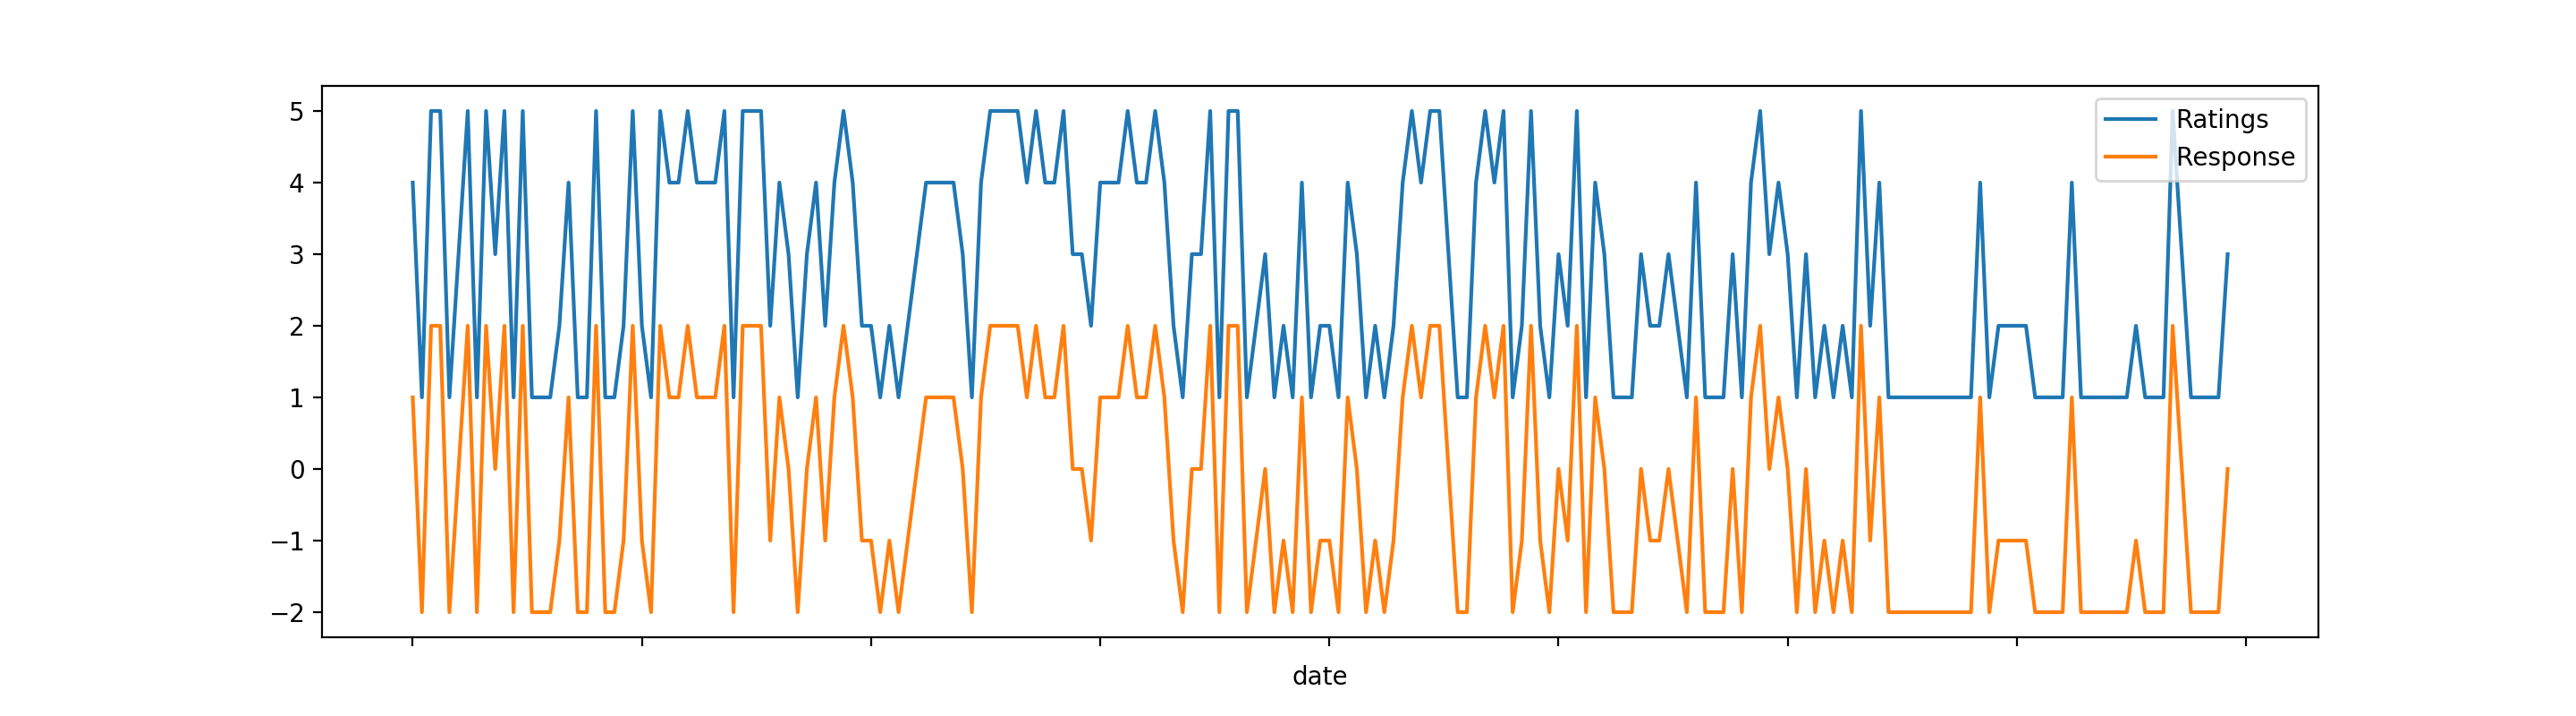
\includegraphics[scale=0.5]{rat_res.png}
\caption{Time series ratings}
\label{fig:rat_res}
\end{figure}

As we can see from the right half of the figure ~\ref{fig:rat_res}, the curve is constant at the bottom. It indicates that most of the people have given 1 star rating after the merger.

\begin{figure}[H]
\centering
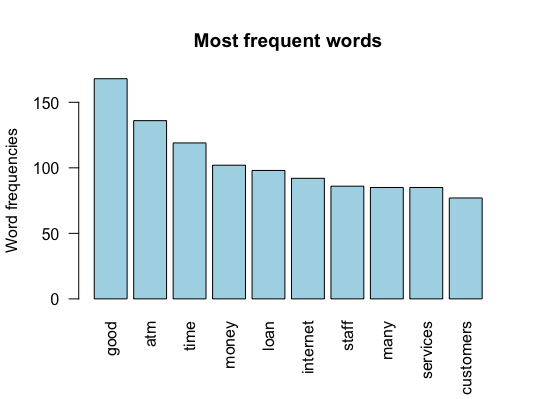
\includegraphics[scale=0.5]{freq_words.png}
\caption{Frequent words in reviews}
\label{fig:freq_words}
\end{figure}

Figure ~\ref{fig:freq_words} shows the top 10 frequent words found in reviews. They are good, atm, time, money, loan, internet, staff, services, customers.


\subsubsection{WORD CLOUD - REVIEWS}
\begin{figure}[H]
\centering
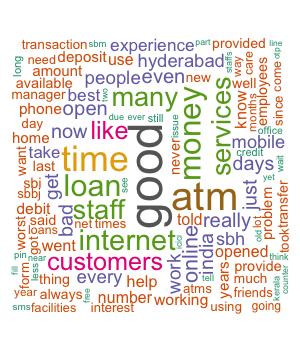
\includegraphics[scale=1]{wordcloud_reviews.png}
\caption{Reviews word cloud}
\end{figure}

\par A word cloud is a novelty visual representation of text data, typically used to depict keyword metadata (tags) on websites, or to visualize free form text. Tags are usually single words, and the importance of each tag is shown with font size or color. This format is useful for quickly perceiving the most prominent terms and for locating a term alphabetically to determine its relative prominence. When used as website navigation aids, the terms are hyperlinked to items associated with the tag.

From the word cloud it is clear that people have mostly spoken about loan, staff, internet, credit, time transfer etc. It can be inferred from the word cloud there are keywords associated with positivity like best and negative keywords like worst.
\subsection{SENTIMENT ANALYSIS}
\begin{table}[H]
67\% of reviews are positive while 33\% of reviews are negative. This shows that customers were generally positive while expressing their concern about the bank.
\centering
\begin{tabularx}{\linewidth}{|X|X|}
\hline Polarity & Percentage\\
\hline Positive & 67 \% \\
\hline Negative & 33 \% \\
\hline
\end{tabularx}
\caption{SENTIMENT ANALYSIS}
\label{table:sent_analysis}
\end{table}
\subsection{STOCK PRICE ANALYSIS}
\begin{figure}[H]
\centering
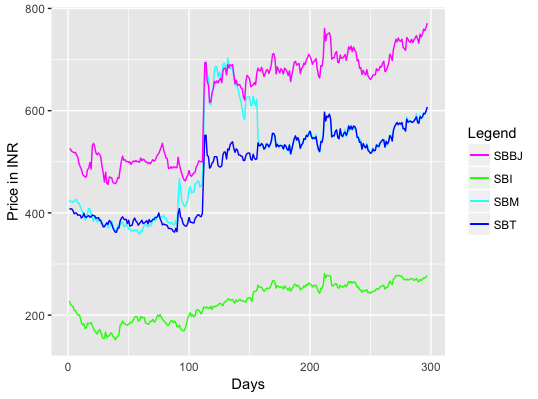
\includegraphics[scale=0.8]{price_action.png}
\caption{Price chart of SBI, SBT, SBBJ, SBM before and after merger period}
\label{fig:price_action}
\end{figure}

\par As we can see from the Figure ~\ref{fig:price_action}, there is a huge surge in stock prices when the merger news was announced. Shares of State Bank of India (BSE) -2.01 \% (SBI) and its three of its listed associates jumped up to 14 per cent. The merger will bring nearly a quarter of all outstanding loans in India's banking sector to SBI?s books.

SBI jumped over 3 per cent to hit a high of Rs 277 on BSE. State Bank of BikanerNSE 0.99 \% \& Hyderabad (SBBJ) soared 10.86 per cent to hit a high of Rs 796. State Bank of Travancore 1.34 \% (SBT) surged 10.54 per cent to Rs 619. State Bank of MysoreNSE 1.17 \% spurted 13.54 per cent to Rs 637.70. SBI holded a 75 per cent stake in SBBJ, 90 per cent in State Bank of Mysore and 79 per cent in SBT before the associate banks were delisted. After that while the prices of 3 listed associate banks remained more or less constant, prices of SBI continues to rise. On march 17, 2017 the associate banks were delisted from both BSE and NSE. The board of SBI earlier approved the merger plan under which SBBJ shareholders will get 28 shares of SBI (Re1 each) for every 10 shares (Rs10 each) held. Similarly, SBM and SBT shareholders will get 22 shares of SBI for every 10 shares.

\subsubsection{RECOMMENDATION TO BUY SHARES}
\par Banking is a regulated sector and government policies have a tight control over it. So any banking shares should be bought with caution. Though the merger creates a good value for shareholders, it alone cannot be kept in mind for buying the share. Recent PNB scam affected all PSU banks and every PSU share is declining. \textbf{So SBI shares should be bought with caution.}

\subsection{SUMMARY}

The data collected from customers of State Bank of India across the major cities of India were analyzed, hypotheses were tested. Using these interpretations, the summary of findings is discussed in the next Chapter.

%conclusion
\newpage
\section{CONCLUSION}
\subsection{FINDINGS}
The data analyses reveal that merger of State Bank of India with its associate banks has not made much negative impact on its customers. Psychological Contract Breach, Customer Satisfaction and Loyalty is medium while service performance is low.

PCV is very medium. Majority of people claimed that they lost their identities after merger. The number people who found difficult to commute was average and the difficulty in getting information was also average.

Customers feel that service performance before and after merger remains more or less same. They didn't see any drastic improvement in service. SBI continues to be SBI one of the respondent quoted. Majority of the customers felt that employees were rude. They were not courteous. Most of the respondents felt that service had met expectation while the after merger service performance was not ideal.

Now that all the associate banks have merged with SBI, the customer base of the bank has become huge. And so, number of customers visiting the bank has also increased. Customers who previously had to travel long to reach any of the associate bank in which he had account ,can now get his job done at any of the nearby branches of the SBI. For example in pollachi before merger there was SBI and SBT. SBI will always be crowdy, since it's located close to bus stand. After merger considerable crowd has decreased and they go to SBT where there is less crowd. It can be inferred that customer satisfaction is also medium.

Loyalty is also medium indicating that people doesn't become mascots for SBI. Many people claimed that private banks offer far better services than SBI like priority banking etc. They mentioned that some had no other choice other than opening with SBI due to circumstances. If now they are offered an option to switch they will definitely switch to other banks as evident from the descriptive statistics table.

There is no correlation between ratings and reviews. Most of the ratings were 1, indicating a poor review, but reviews didn't correlate with ratings as evident from sentiment analysis. So ratings alone cannot be used to evaluate customer and bank performance.

\subsection{SUGGESTIONS}
\begin{itemize}
\item During offline mode data collection it was found that, only some customers knew about the merger. Some where in the mindset mergers are good and quoted united is good. So customers should be educated about merger by the bank the advantages, the benefits and also disadvantages of merger.
\item As we can see from review analysis and quite a few offline respondents said that the banks in study are good to get loans particularly agri loan. The banks should improve well in other services.
\item Customer satisfaction score is very low 43\%, which is very much less than industry average of 70\%. So bank should should increase customer satisfaction by introducing customer engagement activities.
\item Banks should treat all their customers equally. Only few people said that they didn't loss their identity. So bank should treat every person equally and provide care like private banks.
\item Time and effort taken to receive a service should be reduced.
\item Since most of the people said that they won't open an account again, banking should be made more fun. Gamification should be introduced in banking and more rewards should be provided and customers must be retained.
\end{itemize}
\subsection{CONCLUSION}
Though merger is beneficial to management in terms of financial perspective and synergies, merger often brings a lot of pain to customer. In our case many branches were shut down, customers lost identities etc. So merger should be planned with customer in mind to ensure smooth functioning and service.

\subsection{FUTURE WORK}
During response collection it was found that, many of the people preferred private banks over SBI/PSU banks. So a study can be conducted to know the areas in which private banks excel and it can be used to improve the service of PSU banks.

% appendix

\newpage
\section{APPENDIX}
\subsection{SURVEY QUESTIONNAIRE}
\emph{Dear Sir / Madam, I am a second year MBA student from Anna University, Chennai. We are conducting this survey to know about customer satisfaction and loyalty after merger of associate banks of SBI with itself. There is no right or wrong answer. Please read the statements carefully and answer. All the data will be kept confidential. It will be used only for educational and research purposes only. None of the data will be disclosed.}\\
\noindent\makebox[\linewidth]{\rule{\paperwidth}{0.4pt}}
Age:\\
Gender:\\
Bank Name:\\
Year of account opening:\\
Location:\\
Education:\\
\noindent\makebox[\linewidth]{\rule{\paperwidth}{0.4pt}}

\subsection*{SECTION 1 (PSYCHOLOGICAL CONTRACT VIOLATION)}
\textbf{Please indicate to what extent you agree with the following statements.} \\
1 = Not at all, 2 = Somewhat, 3 = Neutral, 4 = Some extent, 5 = Very great extent\\
\emph {(Tick in the appropriate box)}\\
\begin{minipage}{\textwidth}

\begin{tabular}{|c|l|c|c|c|c|c|}
\hline \multicolumn{2}{|c|}{} & 1 & 2 & 3 & 4 & 5\\
\hline \rownumber & I feel happy about the merger & \tab & \tab & \tab & \tab & \tab \\
\hline \rownumber & I feel pleased about the merger & \tab & \tab & \tab & \tab & \tab \\
\hline \rownumber & I feel disappointed about the merger & \tab & \tab & \tab & \tab & \tab \\
\hline \rownumber & I feel violated about the merger & \tab & \tab & \tab & \tab & \tab \\
\hline \rownumber & I feel grateful about the merger & \tab & \tab & \tab & \tab & \tab \\
\hline \rownumber & I have difficulty in obtaining information post merger. & \tab & \tab & \tab & \tab & \tab \\
\hline \rownumber & I find difficult to commute. & \tab & \tab & \tab & \tab & \tab \\
\hline \rownumber & I lost my personal care / identity after merger. & \tab & \tab & \tab & \tab & \tab \\
\hline
\end{tabular}

\end{minipage}

\newpage
\subsection*{SECTION 2 (SERVICE PERFORMANCE)}
\textbf{Please rate the following statements.}\\
1 = Very High, 2 = High\\
3 = Same,\\
4 = Low, 5 = Very Low\\
\emph {(Tick in the appropriate box)}\\
\begin{minipage}{\textwidth}

\begin{tabularx}{\linewidth}{|l|l|X|X|X|X|X|}
\hline \multicolumn{2}{|c|}{} & 1 & 2 & 3 & 4 & 5\\
\hline \rownumber & Time required to avail a service & \tab & \tab & \tab & \tab & \tab \\
\hline \rownumber & Effort taken to receive a service & \tab & \tab & \tab & \tab & \tab \\
\hline \rownumber & Employees provide consistent service & \tab & \tab & \tab & \tab & \tab \\
\hline \rownumber & Employees are willing and provide service in a timely manner & \tab & \tab & \tab & \tab & \tab \\
\hline \rownumber & Employees are approachable and easy to contact & \tab & \tab & \tab & \tab & \tab \\
\hline \rownumber & Employees are courteous, polite and respectful & \tab & \tab & \tab & \tab & \tab \\
\hline \rownumber & Employees listen and speak to me in  a language I understand & \tab & \tab & \tab & \tab & \tab \\
\hline \rownumber & Employees are trustworthy, honest and believable. & \tab & \tab & \tab & \tab & \tab \\
\hline \rownumber & Employees make effort to understand my needs.  & \tab & \tab & \tab & \tab & \tab \\
\hline \rownumber & Physical facilities and employees are neat and clean. & \tab & \tab & \tab & \tab & \tab \\
\hline \rownumber & The overall ability of bank to satisfy my needs and wants is. & \tab & \tab & \tab & \tab & \tab \\
\hline
\end{tabularx}
\end{minipage}
\begin{minipage}{\textwidth}
\tab \\
\textbf{Please rate the following statements.}\\
1 = Pathetic, 2 = Poor\\
3 = Same,\\
4 = Good, 5 = Excellent\\
\emph {(Tick in the appropriate box)}\\
\begin{tabularx}{\linewidth}{|l|l|X|X|X|X|X|X|X|X|X|}
\hline \multicolumn{2}{|c|}{} & 1 & 2 & 3 & 4 & 5\\
\hline \rownumber & Overall service & \tab & \tab & \tab & \tab & \tab \\
\hline
\end{tabularx}
\end{minipage}
\newpage
\subsection*{SECTION 3 (CUSTOMER SATISFACTION)}
%\begin{minipage}{\textwidth}
\emph {(Tick only one option)}\\
\rownumber. \textbf{Overall satisfaction level}
\begin{todolist}
    \item Very dissatisfied.
    \item Dissatisfied.
    \item Neutral.
    \item Satisfied.
    \item Very satisfied.
\end{todolist}

\rownumber. \textbf{To what extent, service has met expectation ?}
\begin{todolist}
    \item Much worse.
    \item Worse than expectation.
    \item Neutral.
    \item Equal to expectation.
    \item Better than expectation.
\end{todolist}

\rownumber. \textbf{Compare the current service with before merger.}
\begin{todolist}
    \item Very far from ideal.
    \item Far from ideal.
    \item Neutral.
    \item Close to ideal.
    \item Very close to ideal.
\end{todolist} .
%\end{minipage}
\subsection*{SECTION 4 - (LOYALTY)}
\textbf{Please rate the following statements.}\\
1 = Not at all likely, 2 = Not very likely \\
3 = Quite likely, 4 = Very likely\\
\emph {(Tick in the appropriate box)}\\
\begin{minipage}{\textwidth}

\begin{tabularx}{\linewidth}{|l|l|X|X|X|X|}
\hline \multicolumn{2}{|c|}{} & 1 & 2 & 3 & 4\\
\hline \rownumber & Would you recommend to a friend / relatives? & \tab & \tab & \tab & \tab \\
\hline \rownumber & Will you avail service continuosly ?& \tab & \tab & \tab & \tab \\
\hline \rownumber & Will you open account again ? & \tab & \tab & \tab & \tab \\
\hline
\end{tabularx}

\end{minipage}
\tab \\
\textbf{Please rate the following statements.}\\
1 = Strongly disagree, 2 = Disagree \\
3 = Neutral
4 = Agree, 5 - Strongly agree\\
\emph {(Tick in the appropriate box)}\\
\begin{minipage}{\textwidth}

\begin{tabularx}{\linewidth}{|l|l|X|X|X|X|X|}
\hline \multicolumn{2}{|c|}{} & 1 & 2 & 3 & 4 & 5\\
\hline \rownumber & I had a problem or negative experience after merger? & \tab & \tab & \tab & \tab & \tab \\
\hline \rownumber & Given an option to switch, I will switch to other banks. & \tab & \tab & \tab & \tab & \tab \\
\hline
\end{tabularx}

\end{minipage}

\newpage
\subsection{REFERENCES}
\begin{enumerate}
%\item \href{http://www.thehindu.com/business/Industry/sbi-five-associate-banks-bmb-merge-with-sbi/article17757316.ece}{http://www.thehindu.com/business/Industry/sbi-five-associate-banks-bmb-merge-with-sbi/article17757316.ece}
%\item \href{https://en.wikipedia.org/wiki/Public_sector_banks_in_India}{https://en.wikipedia.org/wiki/Public-sector-banks-in-India}
%\item \href{https://www.ukessays.com/essays/economics/advantages-and-disadvantages-of-mergers-and-acquisition-economics-essay.php}{https://www.ukessays.com/essays/economics/advantages-and-disadvantages-of-mergers-and-acquisition-economics-essay.php}
%\item \href{https://www.quora.com/in/What-is-the-reason-behind-SBI-associate-banks-merger-What-could-be-its-pros-and-cons}{https://www.quora.com/in/What-is-the-reason-behind-SBI-associate-banks-merger-What-could-be-its-pros-and-cons}
\item Rousseau, D. M., \& Tijoriwala, S. A. (1998). Assessing psychological contracts: Issues, alternatives, and measures. Journal of Organizational Behavior, 19(1)%, 679?695
\item Rousseau, D. M. (1995). Psychological contracts in organizations. Understanding written and unwritten agreements. Thousand Oaks, CA: Sage
\item Theotokis, A., Pramatari, K., \& Tsiros, M. (2012). Effects of expiration date-based pricing on brand image perceptions. Journal of Retailing%, 88(1), 72?87.
\item Neeru Malhotra, Sunil Sahadev, \& Keyoor Purani (2017).Psychological contract violation and customer intention to reuse online retailers: Exploring mediating and moderating mechanisms. Journal of Business Research%, 75 (2017) 17?28	.
\item Pavlou, P. A., \& Gefen, D. (2005). Psychological contract violation in online marketplaces: Antecedents, consequences, and moderating role. Information Systems Research%, 16(4), 372?399.
\item Robinson, S.L., Morrison, E.W., 2000. The development of psychological contract breach and violation: a longitudinal study. Journal of Organizational Behavior %21 (5), 525?547
\item Morrison, E.W., Robinson, S.L., 1997. When employees feel betrayed: a model of how psychological contract violation develops. Academy of Management Review% 22 (1), 226?256
\item Wang, S., \& Huff, L. C. (2007). Explaining buyers' responses to sellers' violation of trust. European Journal of Marketing%, 41(9/10), 1033?1052
\item Bagozzi, R., Gopinath, M., \& Nyer, P. (1999). The role of emotions in marketing. Journal of the Academy of Marketing Science%, 27(2), 184?206
\item James A. Hill, Stephanie Eckerd, Darryl Wilson, Bertie Greer .,(2008). The effect of unethical behavior on trust in a buyer-supplier relationship: The mediating role of psychological contract violation. Journal of Operations Management.% 27 (2009) 281?293
\item Freese, Hogeschool, Bosch. How to measure the psychological contract? A critical criteria-based review of measures.South African Journal of Psychology
\item Danaher \& Haddrell (1996). A comparison of question scales used for measuring customer satisfaction. International Journal of Service Industry Management
\item  Angelova \& Zekiri (2011). Measuring Customer Satisfaction with Service Quality Using American Customer Satisfaction Model (ACSI Model). International Journal of Academic Research in Business and Social Sciences 
\item Cronin,Brady, G.Thomas, M Hult (2000). Assessing the Effects of Quality, Value, and Customer Satisfaction on Consumer Behavioral Intentions in Service Environments. Journal of Retailing 
\item Yuksel, Yuksel, Blim (2009). Destination attachment: Effects on customer satisfaction and cognitive,affective and conative loyalty.
\item Bastos, J A.R., and Gallego, P.M (2008). Pharmacies Customer Satisfaction and Loyalty: A Framework Analysis. Journal of Marketing. Universidad de Salamanca
\item Hallowell, R. (1996). The relationships of customer satisfaction, customer loyalty and profitability: An empirical study. International Journal of Service Industry Management, Vol. 7 No. 4, pp. 27-42.
\item Giese, J. L. and Cote, J.A (2002). Defining Consumer Satisfaction. Academy of Marketing Science Review
\item Kumar V. Shah D. (2004). Building and sustaining profitable customer loyalty for the 21st century. journal of Retailing
\item Nadiri, H., Hussain, K., Ekiz, E. H. Erdogan S. (2008). An investigation on the factors influencing passengers? loyalty in the North Cyprus national airline. The TQM Journal. Vol. 20 (3)
\item Lak, Turekten. (2014). Customer ratings vs Sentiment analysis. A comparison of explicit and implicit measure of opinions. Hawaii International Conference on System Science.
\end{enumerate}
}
\end{document}